\section*{Soft Tasks}
\subsection*{Correlation Analysis}

To investigate correlations in the OSM dataset, we programmed a combined visualization called ``Pub Crawl'', which shows the average minimum inter-pub distance and the average minimum pub to ATM distance within each administrative area (with more than one pub and at least one ATM). The dimensions were mapped to hue and saturation, respectively, allowing us to visualize them both via polygon color. The two measures don't seem to be strongly correlated, but the visualization might be useful for anyone planning to go bar-hopping in the capital.

\begin{figure}
\centering
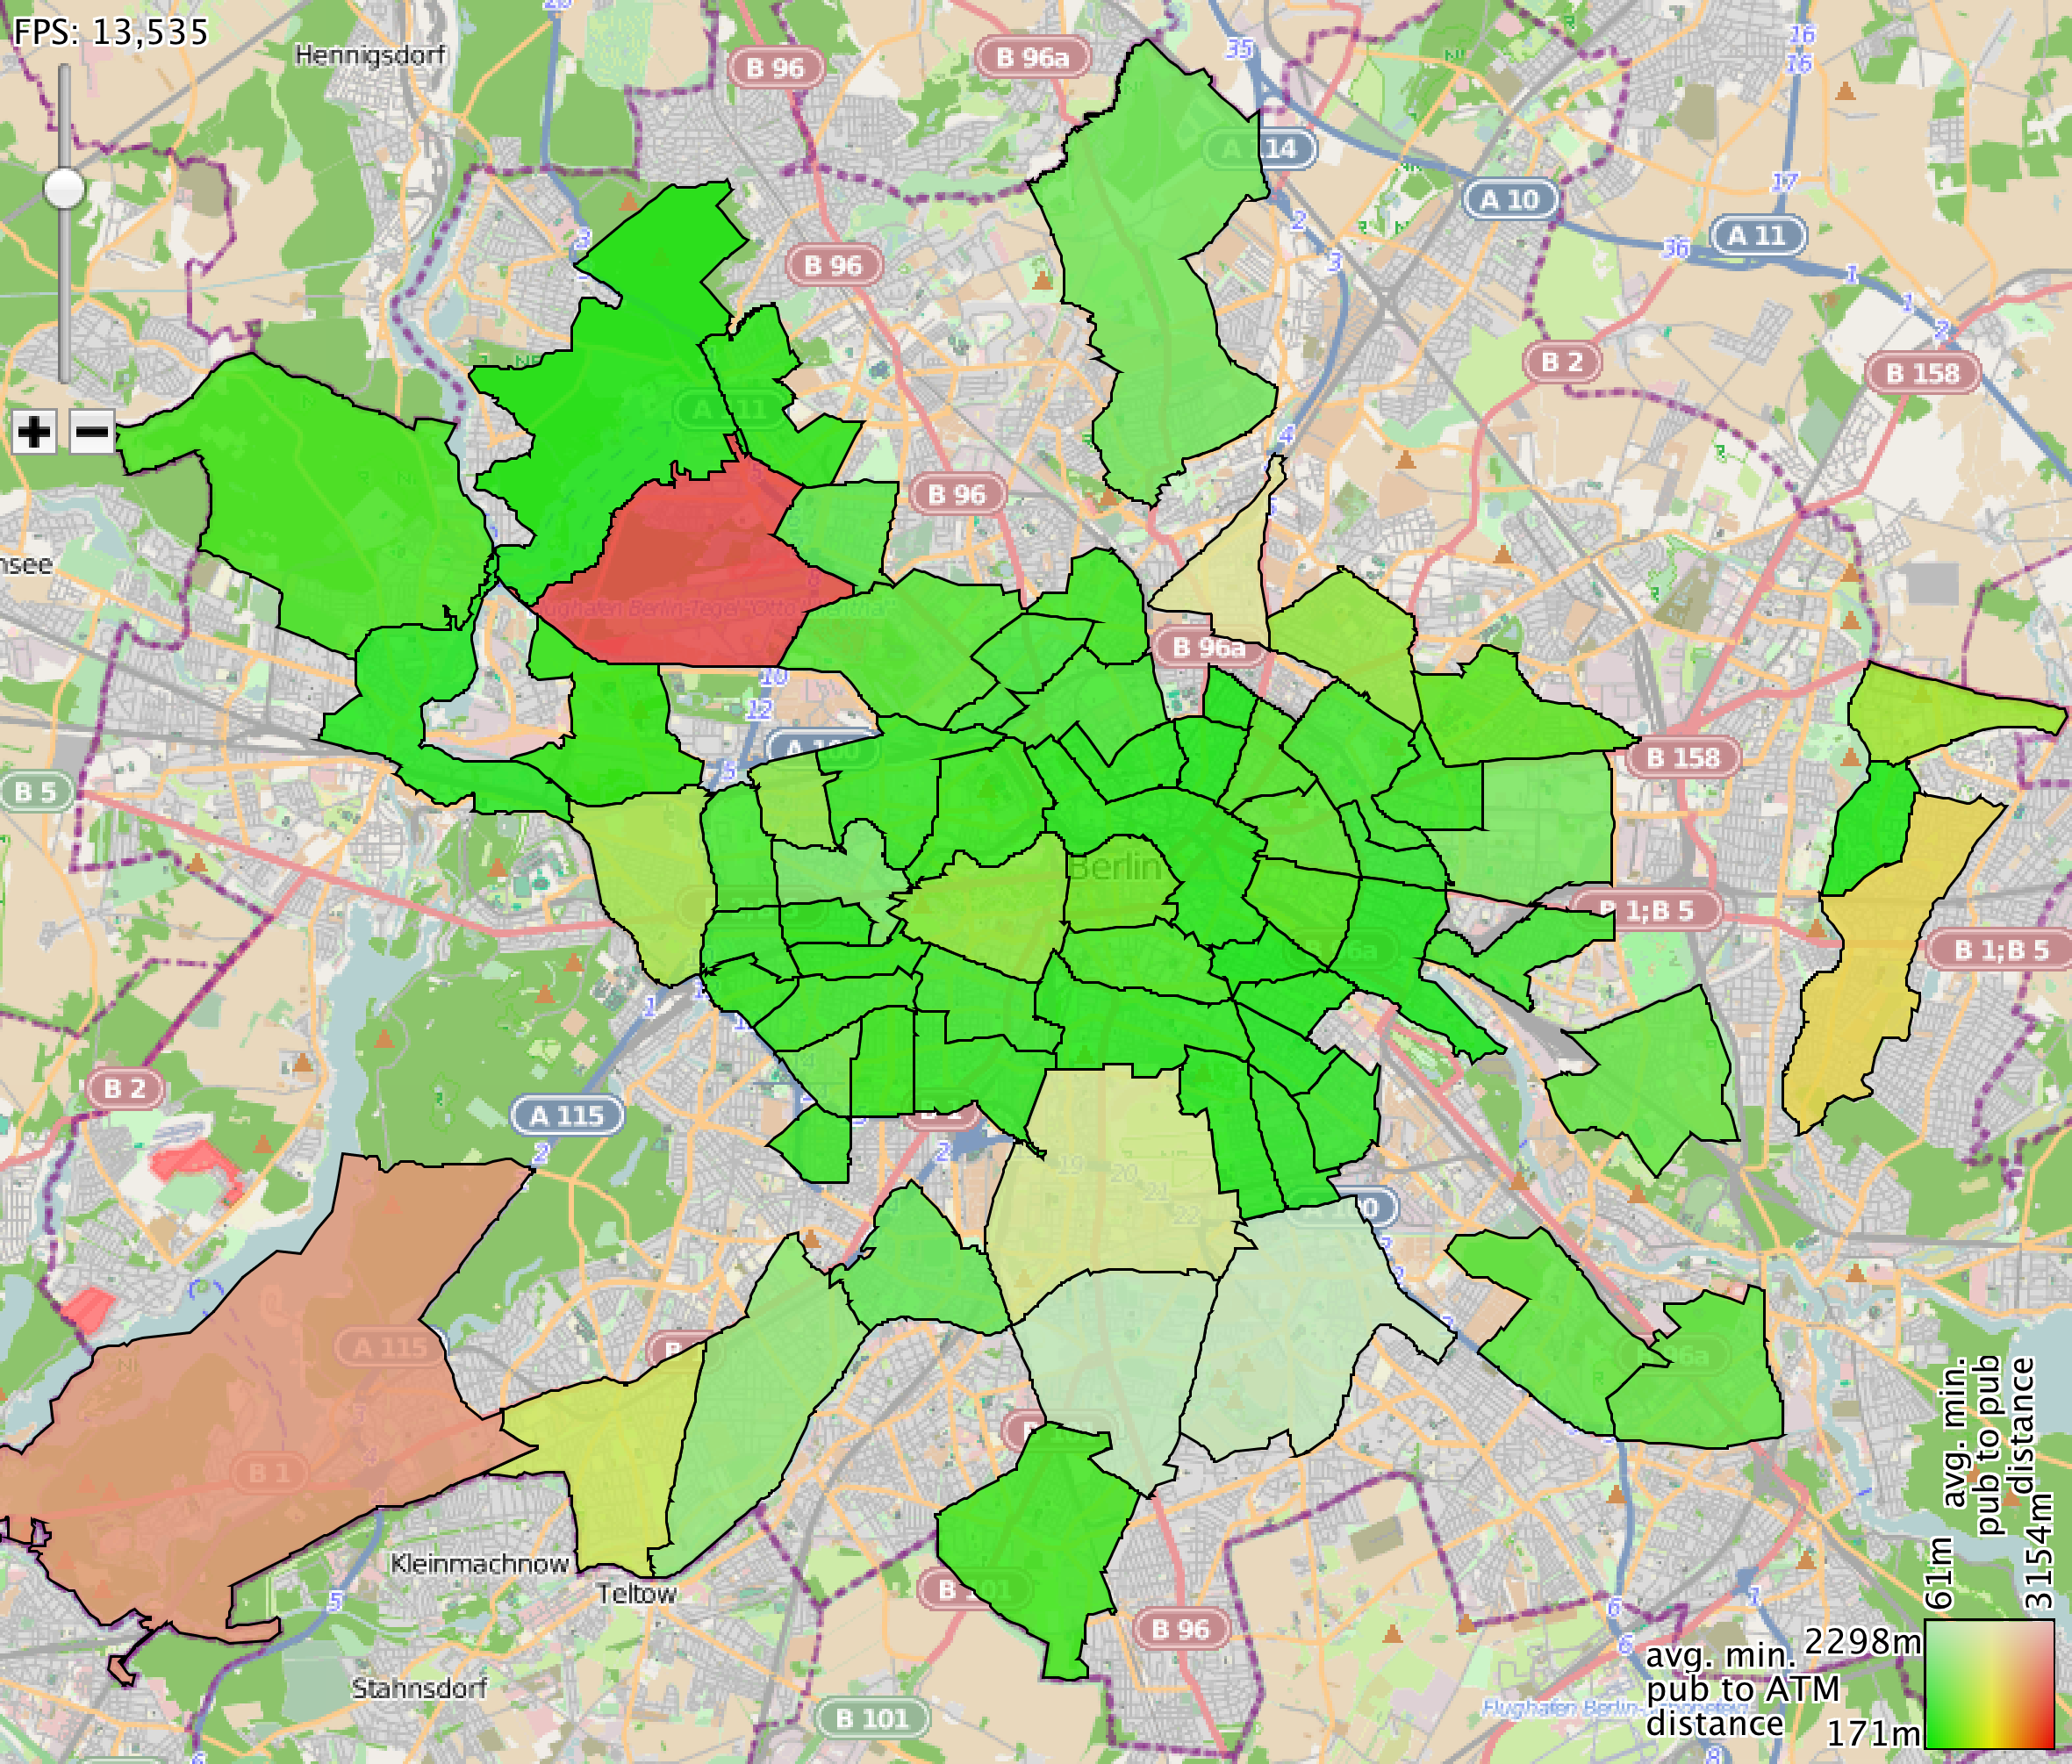
\includegraphics[width=0.9\linewidth]{imgs/crawl}
\caption{\todo{}}
\label{fig:crawl}
\end{figure}

\subsection*{Open Wi-Fi}

As additional dataset we use data of open and free Wi-Fi hotspots in
the area of Berlin.
The data is displayed as a heatmap.

The dataset originally consisted only of plain-text street addresses
of public institutions, hotels, bars, restaurants, coffee places, and other businesses with open Wi-Fi hotspots. We had used the Google geocoding API to retrieve street addresses for all buildings from the given dataset, based on the buildings' centroids. Wireless hotspots were then assigned to buildings by matching addresses between the two datasets.

The heatmap is computed in a mesh of
arbitrary size. Each cell is computed by adding
the nearest distances of all buildings with a Wi-Fi
hotspot together.
Since this is computationally expensive ($\mathcal{O}(whn)$ where $w$ and $h$
are the width and height of the mesh respectively and $n$ is the total number of lines
defining all buildings with Wi-Fi)
we start with a loose mesh and refine it up to one pixel per cell while the
user is inactive.

Looking at the heatmap reveals some areas with higher density of open hotspots.
Namely the center of the city (Mitte), around the Sony Center, in Prenzlauer Berg, and
in the area around Simon-Dach-Str. in Friedrichshain and around Kürfürstendamm in Wilmersdorf.
Those areas are known for being touristic and Mitte with Sony Center are additionally
areas with many businessmen.
As hotspots are likely to be in a restaurant, bar, or caf\'{e}
this seems to be due to the high demand for internet
of tourists (having no alternative) and businessmen (needing to
be online during lunch).

\begin{figure}
\centering
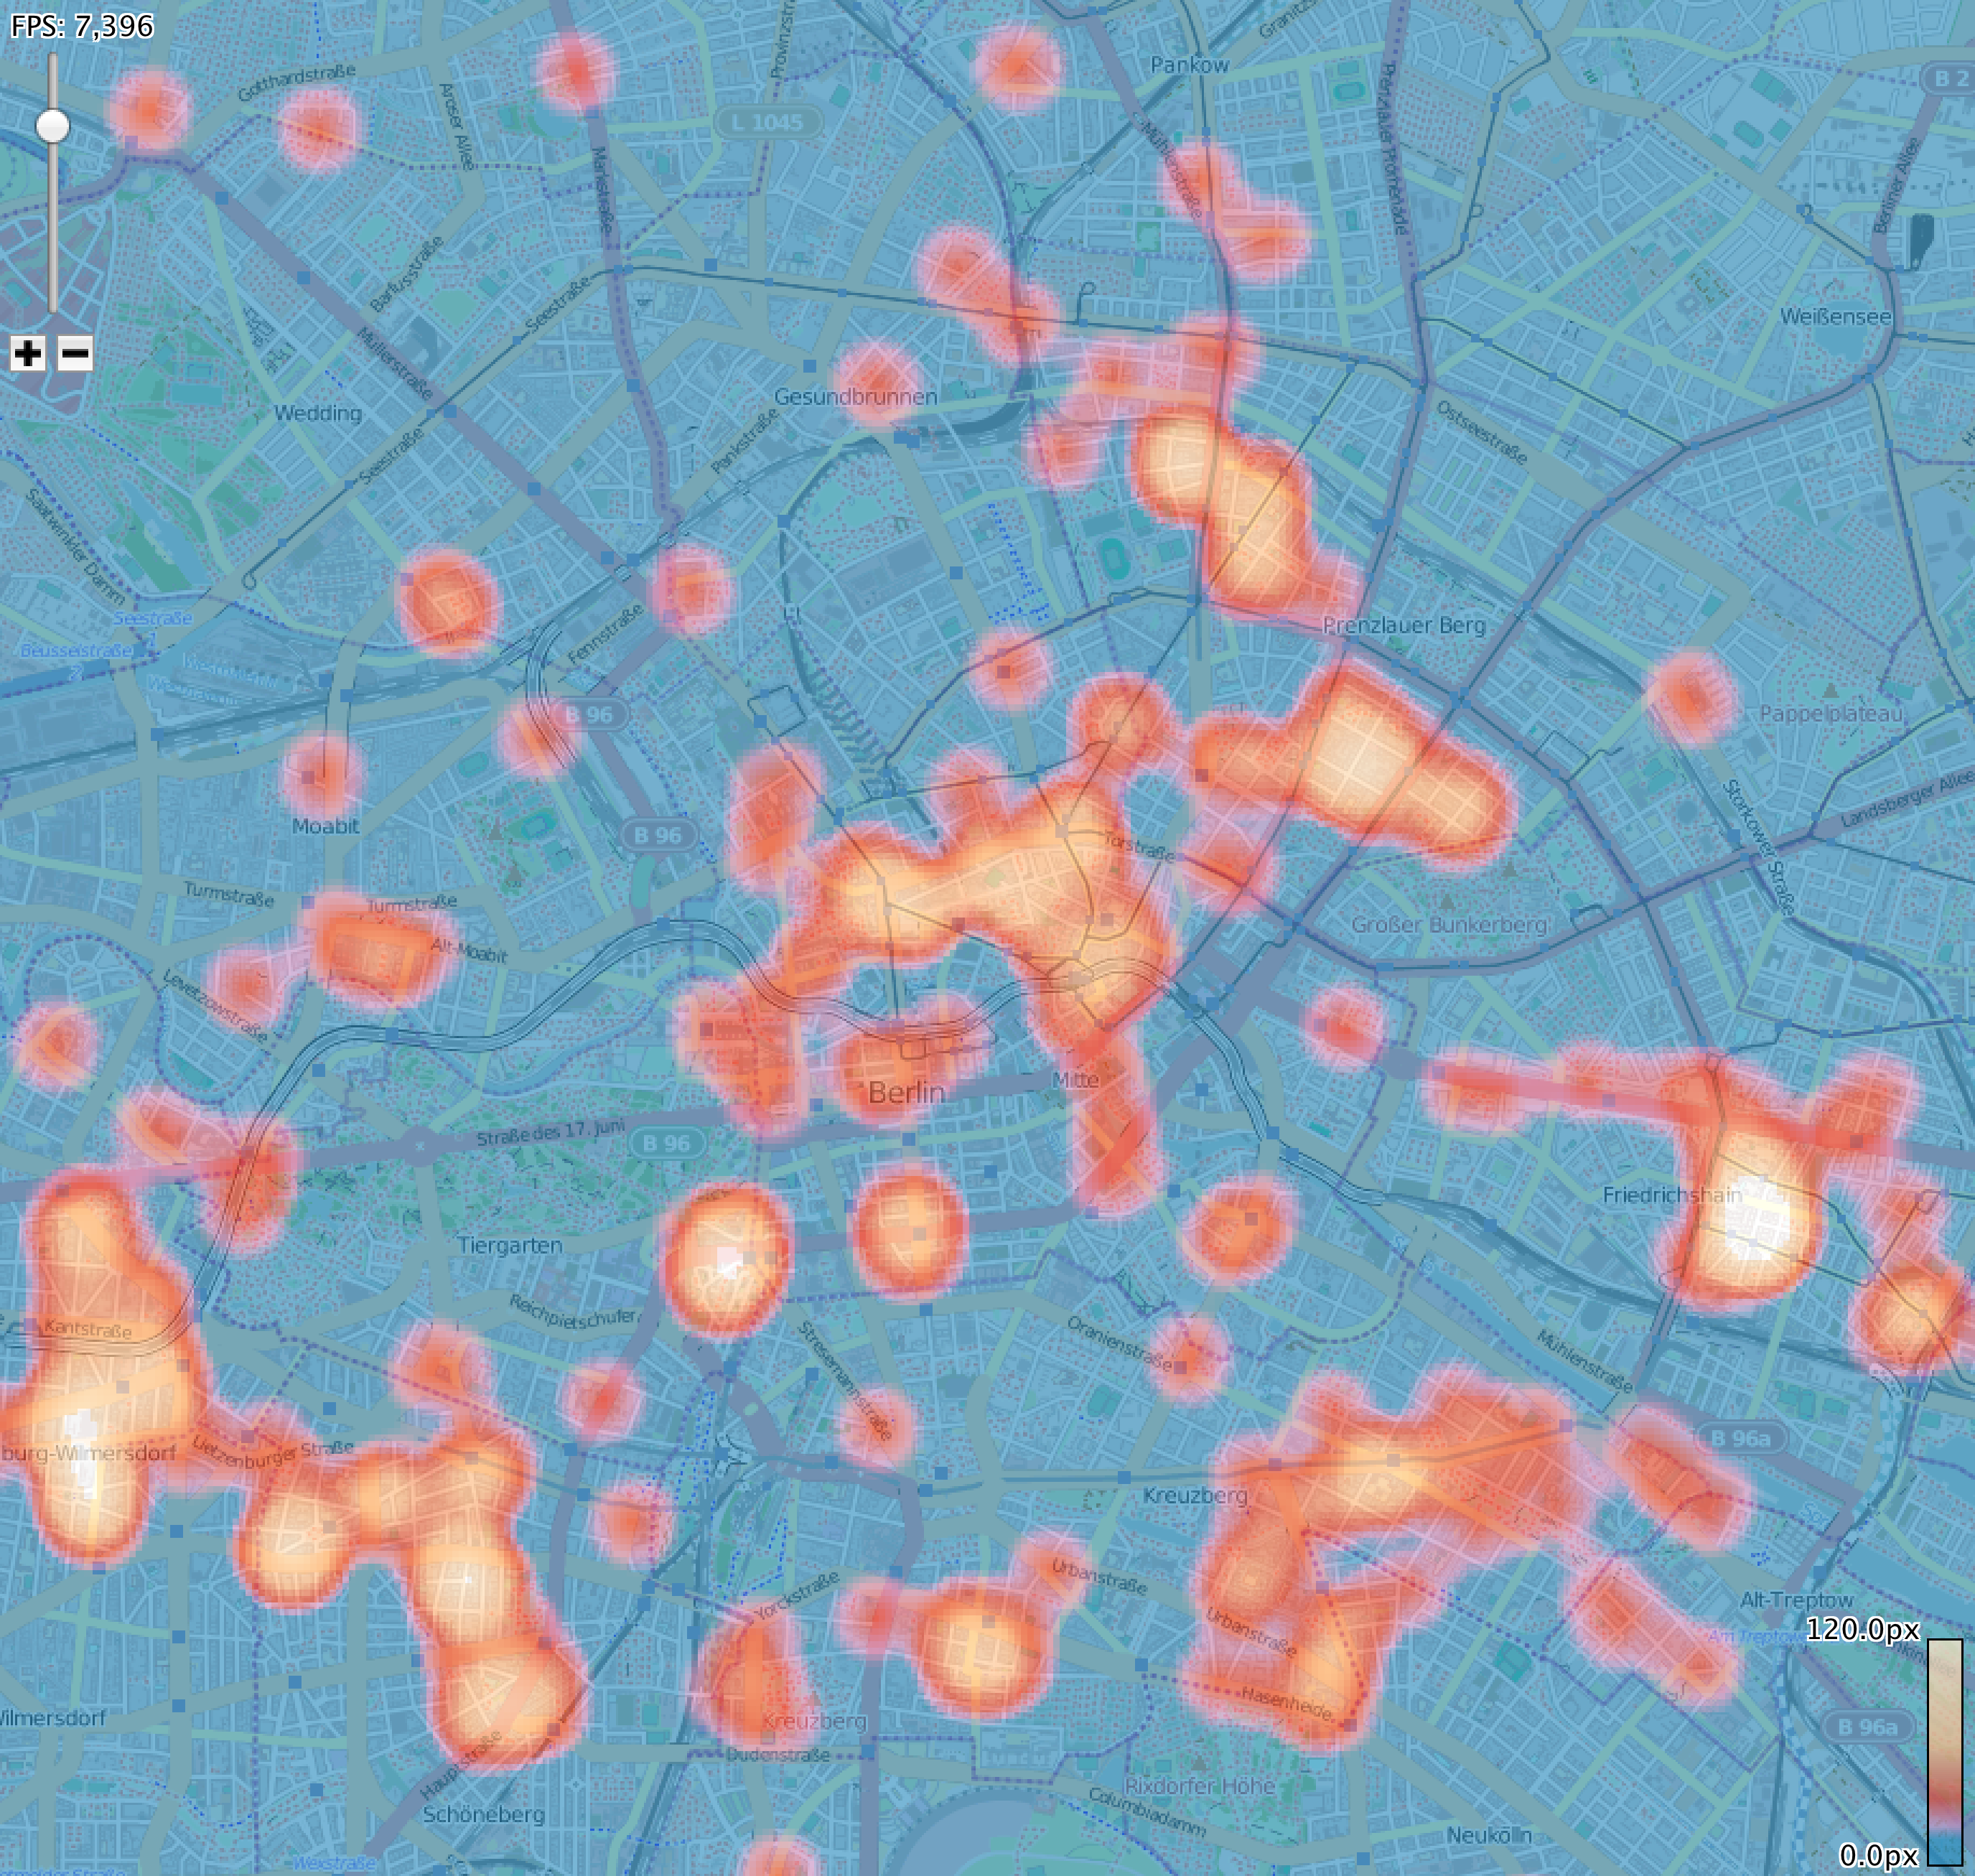
\includegraphics[width=0.9\linewidth]{imgs/heat}
\caption{The heatmap of free hotspots in Berlin.
The white spot to the right is the area around Simon-Dach-Str.}
\label{fig:heat}
\end{figure}

Based on our visualization of the hotspot data, we hypothesized that the hotspot locations are unevenly distributed, with a greater density near the city center. To investigate this further, we computed a distribution of the hotspots w.r.t. their distance from the centroid of Berlin and compared it to the distribution that would result from a uniform hotspot density all over Berlin. Both distributions are visualized as step functions in Fig.~\ref{fig:wifi_distributions}. Although this simple approach does not permit conclusions regarding the significance of the apparent differences, it does provide support for our hypothesis.

\begin{figure}[tbp]
	\centering
	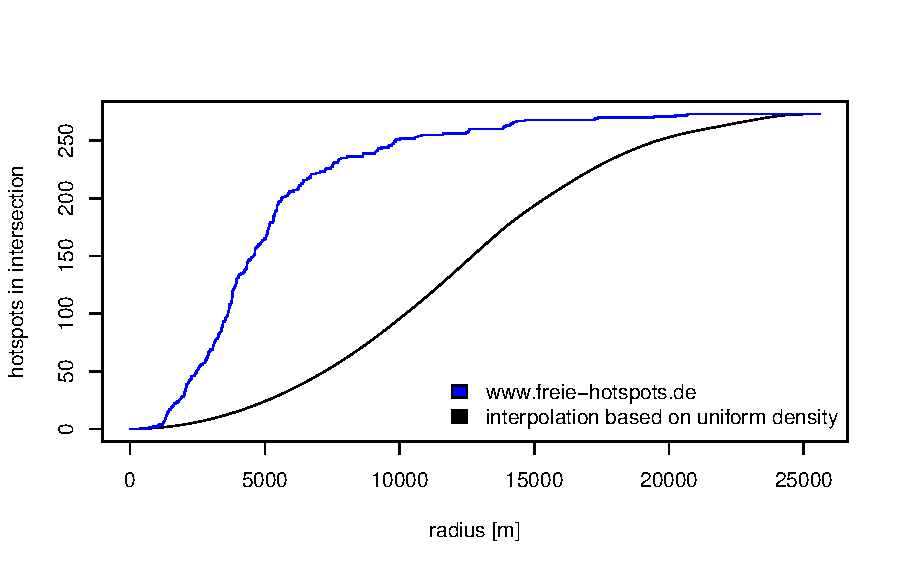
\includegraphics[scale=0.6]{imgs/wifi_distributions.pdf}
	\caption{Number of hotspots within (varied) distances around the centroid of Berlin.}
	\label{fig:wifi_distributions}
\end{figure}
